\documentclass{article}

\title{Zumobot case study}
\date{29.6.2017}
\author{Javier Reyes}

\usepackage{graphicx}
\usepackage{booktabs}

\usepackage[backend=biber, style=numeric]{biblatex}
\bibliography{base}


\begin{document}

\maketitle
\pagenumbering{gobble}
\newpage
\pagenumbering{arabic}

\tableofcontents
\newpage

\section{Introduction}

One of the most used study cases in Control Theory is the Inverted Pendulum analysis, as it present an unstable open-loop characteristic but is also possible to stabilize on a closed-loop configuration.

Here we present the anyalis of the Zumobot 32U4, a small robot available on the market. It is equiped with two DC motors, an Arduino-based board with several periferials.

\section{System analysis}

An inverted pendulum can be represented as a cart moving on an horizontal axis, connected to a rigid body pendulum.

\begin{figure}[h!]
	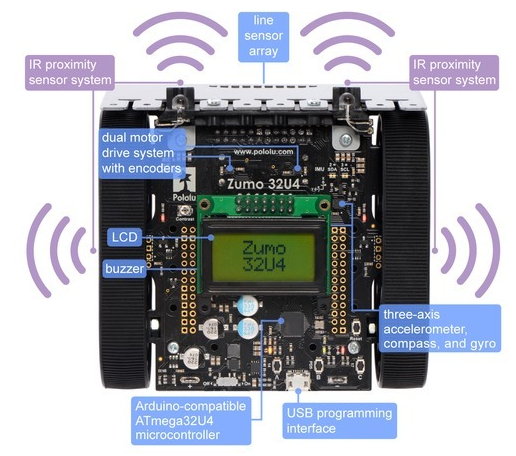
\includegraphics{img/zumo-superior.png}
	\centering
	\caption{Superior view of the zumo robot.}
	\label{fig:sup-zumo}
\end{figure}

The figure \ref{fig:sup-zumo} shows the robot that will be modeled as a Wheeled Inverted Pendulum.

\begin{table}[h!]
	\centering
	\caption{Basic table.}
	\label{tab:tab1}
	\begin{tabular}{ccc}

		\toprule

		header A & header B & header C\\

		\midrule

		a & b & c\\
		c & d & e\\
		f & g & h\\

		\bottomrule

	\end{tabular}
\end{table}

Text of the section\footnote{\label{fn1}This is a footnote}.

Text of the section after the footnote \ref{fn1}.

\section{Mathematical development}

Through the literature is possible to find several approaches to obtain a model for the IP.

To fully model the dynamic behavior of the zumo robot, we need to consider the equations that govern the movement as rigid body.

Text of the section\cite{DOE17} with a reference.

Text of the section\cite{TYSON08} with another reference.

\section{System model}

Text of the section.

\section{Regulator}

Text of the section.

\section{Implementation}

Text of the section.

\begin{appendix}
	\newpage
	\listoffigures
	\newpage
	\listoftables
\end{appendix}

\newpage
\printbibliography

\end{document}
